\documentclass[xcolor=dvipsnames,aspectratio=169]{beamer}
\usecolortheme[dark,accent=cyan]{solarized}
\usepackage[utf8]{inputenc}
\usepackage{multicol}
\usepackage{url}
\usepackage{hyperref}
\usepackage{subfig}
\title{Cryptography}
\author{Gaspare Ferraro\\ ferraro@gaspa.re}
\subtitle{Hackers ahead of time}

\begin{document}

\begin{frame}[plain]
\maketitle
\begin{columns}
\column{0.5\textwidth}
	\center {
		
\includegraphics[width=0.3\textwidth]{style/qrcode.png}\\
		Visit us!
		}
\column{0.5\textwidth}
	\center{
		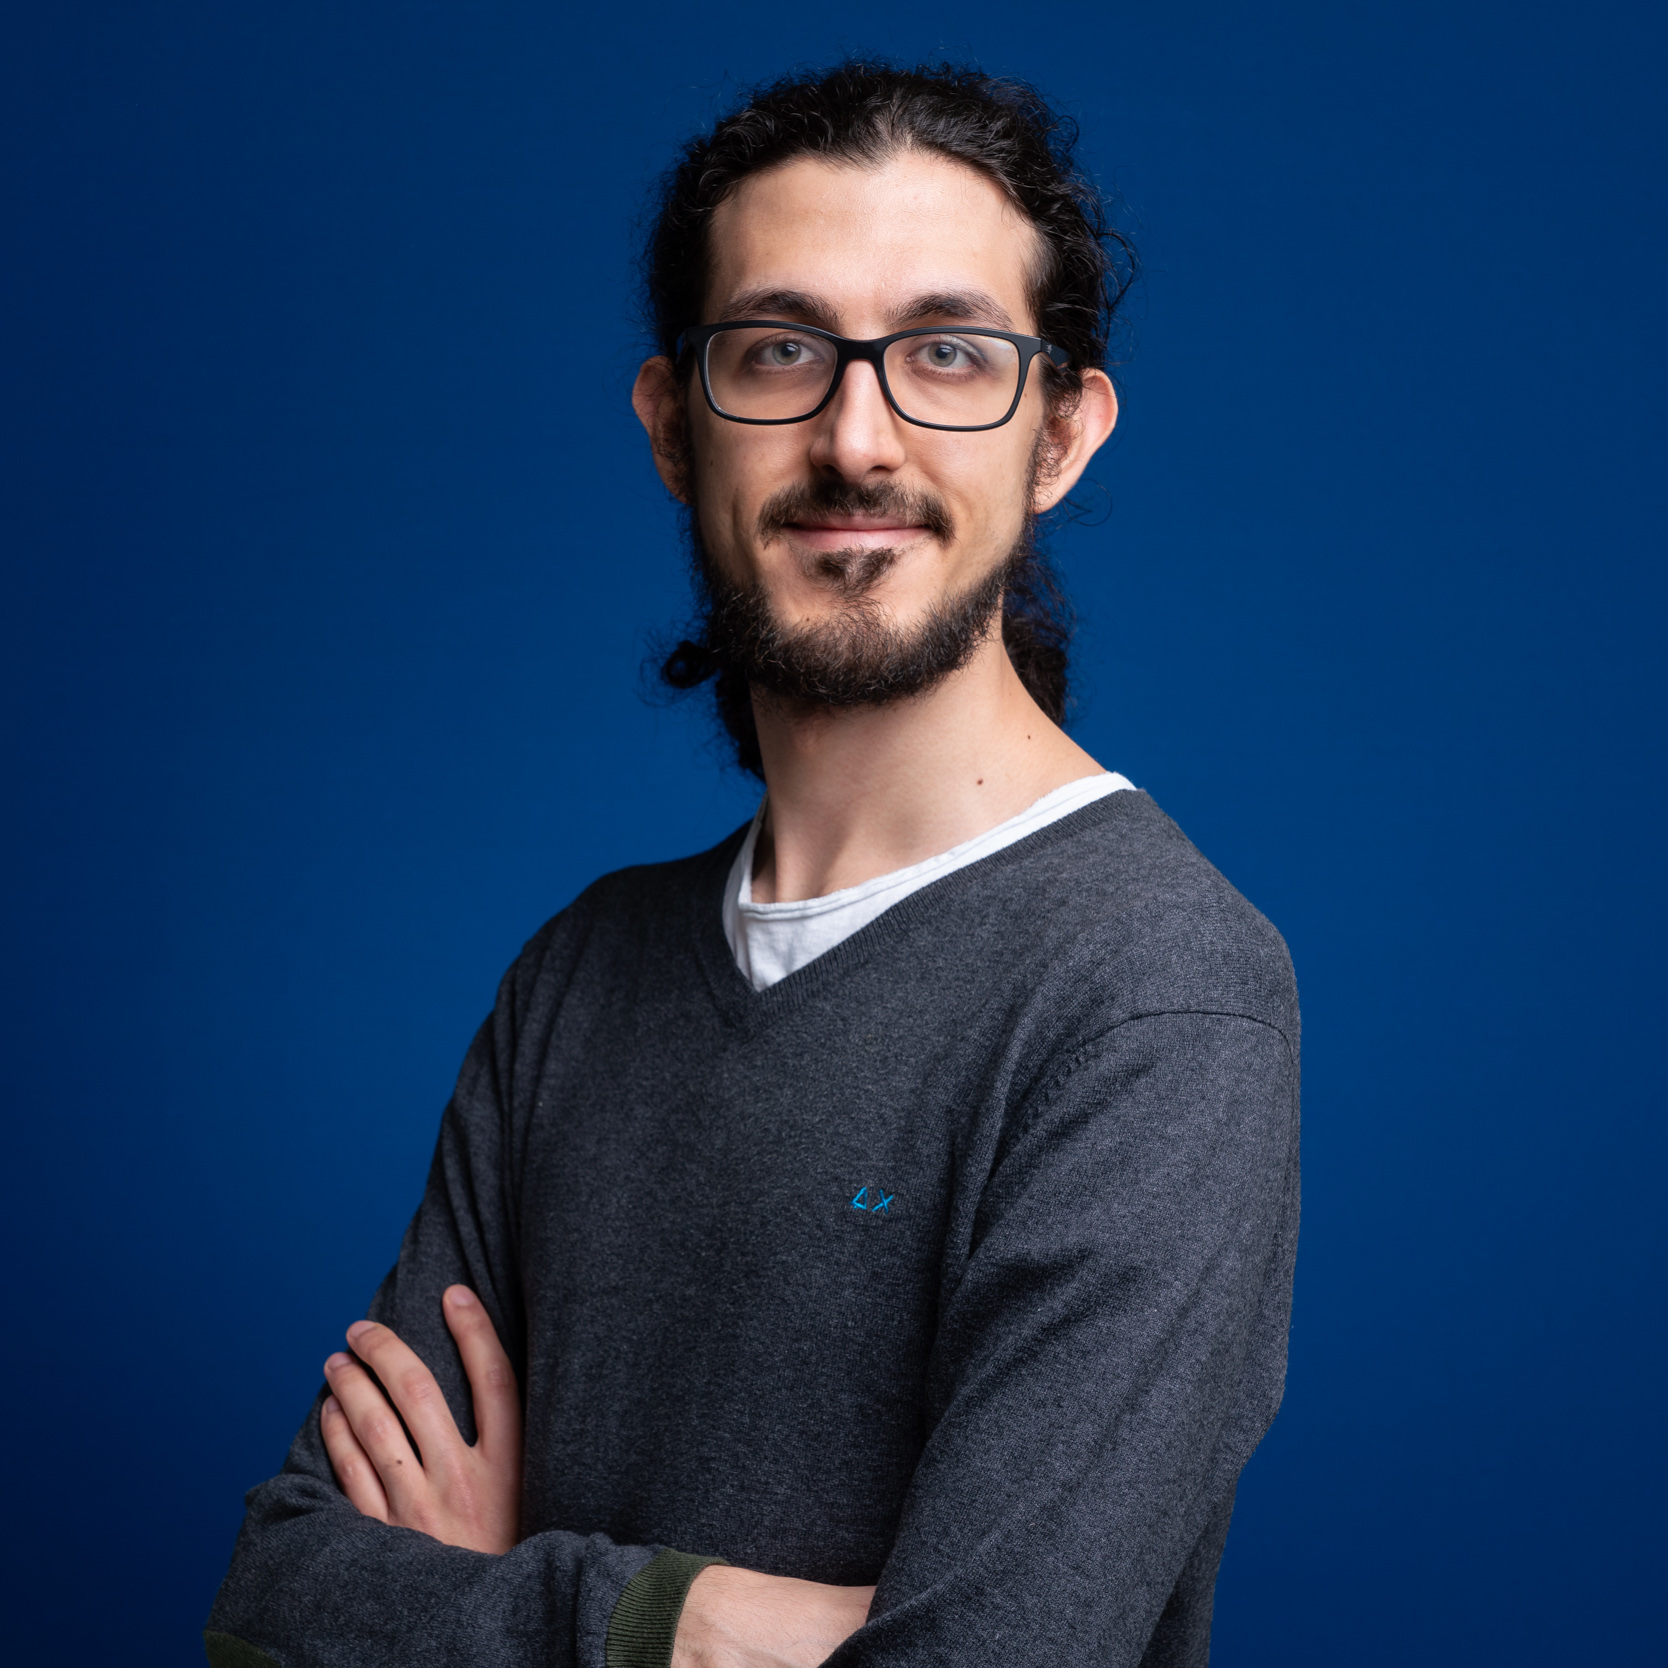
\includegraphics[width=0.3\textwidth]{style/gaspare.jpg}\\
		@GaspareG
	}
	
\end{columns}
\end{frame}

%%%%%%%%%%%%%%%%%%%%%%%%%%%%%%%%%%%%%%%%%%%%%%%%%%%%%%%%%%%%%%%%%%%%%%%%%%%%%%%
%%%%%%%%%%%%%%%%%%%%%%%%%%%%%%%%%%%%%%%%%%%%%%%%%%%%%%%%%%%%%%%%%%%%%%%%%%%%%%%

\part{Introduzione}

\begin{frame}
	\partpage
	\centering
\end{frame}

\begin{frame}{Warning!}

  \center {
    In questo incontro si fa uso della {\color{red} \textit{matematica}}! 
    
    \medskip
    
    \pause

    
\includegraphics[width=0.5\textwidth]{img/meme}
    
    \medskip
    
    \pause

    Non è sempre stato così però...
  }
  
\end{frame}

\begin{frame}{La crittografia ieri}
    
  \pause

  \begin{figure}%
    \centering
    \subfloat[Cifrario di Cesare]{{
  \centering
\includegraphics[width=5cm]{img/cesaer.png} }}%
  \pause
    \qquad
    \subfloat[Scitala]{{
  \centering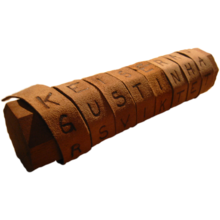
\includegraphics[width=5cm]{img/scitala.png} }}%
    %\caption{2 Figures side by side}%
    %\label{fig:example}%
  \end{figure}


\end{frame}

\begin{frame}{La crittografia oggi}
  \center {
    Le necessità, così come le risorse a disposizione, si sono evolute 
    
    ed oggi possiamo suddividere la crittografia in:
     
    \pause
    
    \medskip
    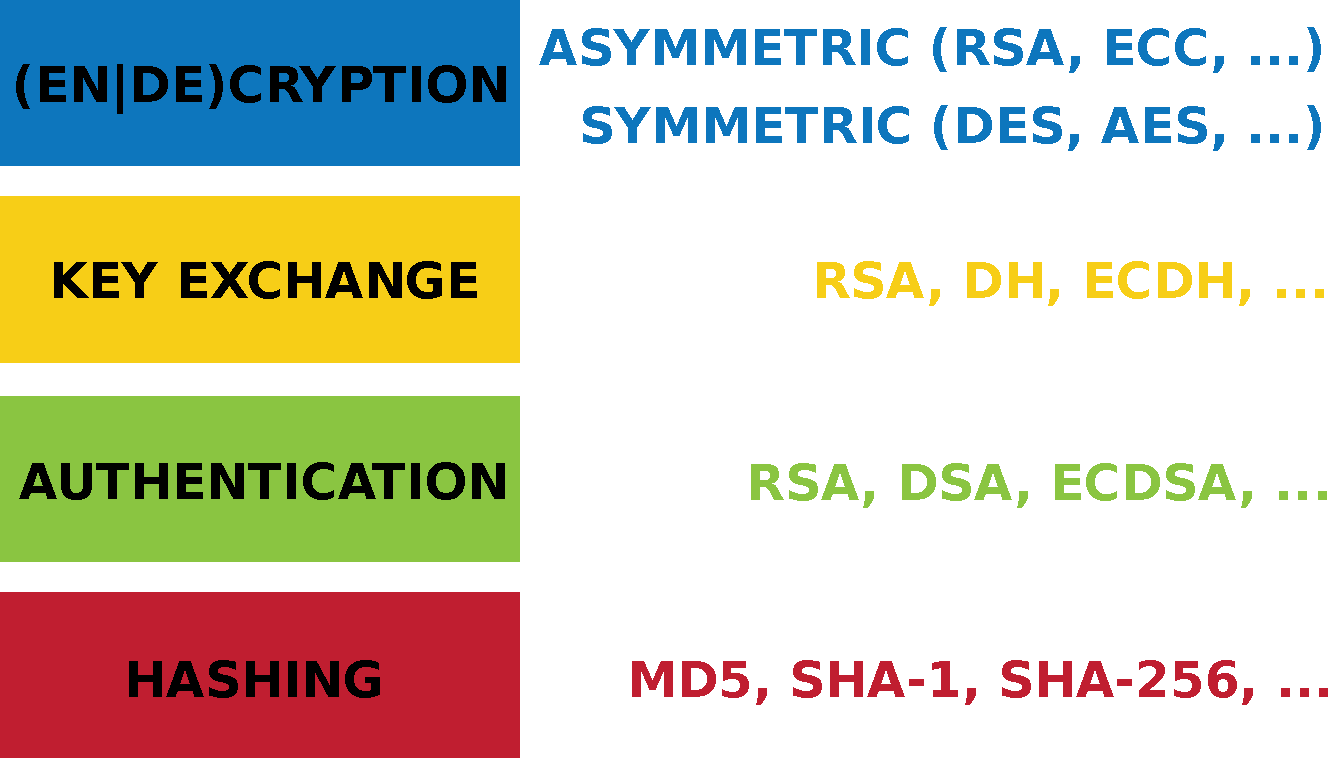
\includegraphics[width=0.6\textwidth]{crypto-section.pdf}
  }
\end{frame}
%%%%%%%%%%%%%%%%%%%%%%%%%%%%%%%%%%%%%%%%%%%%%%%%%%%%%%%%%%%%%%%%%%%%%%%%%%%%%%%
%%%%%%%%%%%%%%%%%%%%%%%%%%%%%%%%%%%%%%%%%%%%%%%%%%%%%%%%%%%%%%%%%%%%%%%%%%%%%%%

\part{Crittografia simmetrica}

\begin{frame}
	\partpage
	\centering
\end{frame}

\begin{frame}
  
\end{frame}

%%%%%%%%%%%%%%%%%%%%%%%%%%%%%%%%%%%%%%%%%%%%%%%%%%%%%%%%%%%%%%%%%%%%%%%%%%%%%%%
%%%%%%%%%%%%%%%%%%%%%%%%%%%%%%%%%%%%%%%%%%%%%%%%%%%%%%%%%%%%%%%%%%%%%%%%%%%%%%%

\part{Crittografia asimmetrica}

\begin{frame}
	\partpage
	\centering
\end{frame}

%%%%%%%%%%%%%%%%%%%%%%%%%%%%%%%%%%%%%%%%%%%%%%%%%%%%%%%%%%%%%%%%%%%%%%%%%%%%%%%
%%%%%%%%%%%%%%%%%%%%%%%%%%%%%%%%%%%%%%%%%%%%%%%%%%%%%%%%%%%%%%%%%%%%%%%%%%%%%%%

\part{Hashing}

\begin{frame}
	\partpage
	\centering
\end{frame}

%%%%%%%%%%%%%%%%%%%%%%%%%%%%%%%%%%%%%%%%%%%%%%%%%%%%%%%%%%%%%%%%%%%%%%%%%%%%%%%

\end{document}
